\documentclass[11pt]{article}
\usepackage[margin=1in]{geometry}
\usepackage{graphicx}
\usepackage{float}
\usepackage{booktabs}
\usepackage{siunitx}
\usepackage{amsmath}
\usepackage{amssymb}
\usepackage{pgfplots}
\usepackage{listings}
\usepackage{xcolor}

% PGFPlots configuration
\pgfplotsset{compat=1.18}
\pgfplotsset{
  standard/.style={
    width=0.85\textwidth,
    height=0.45\textwidth,
    grid=both,
    grid style={line width=.1pt, draw=gray!20},
    major grid style={line width=.2pt,draw=gray!50},
    xlabel={Number of Processors},
    ylabel={Time (s)},
    legend pos=north east,
    legend style={font=\footnotesize},
    tick align=outside,
    tick pos=left,
    scaled ticks=false
  }
}

% Code listing style
\definecolor{codegreen}{rgb}{0,0.6,0}
\definecolor{codegray}{rgb}{0.5,0.5,0.5}
\definecolor{codepurple}{rgb}{0.58,0,0.82}
\definecolor{backcolour}{rgb}{0.95,0.95,0.92}

\lstdefinestyle{mystyle}{
  backgroundcolor=\color{backcolour},
  commentstyle=\color{codegreen},
  keywordstyle=\color{magenta},
  numberstyle=\tiny\color{codegray},
  stringstyle=\color{codepurple},
  basicstyle=\ttfamily\footnotesize,
  breakatwhitespace=false,
  breaklines=true,
  captionpos=b,
  keepspaces=true,
  numbers=left,
  numbersep=5pt,
  showspaces=false,
  showstringspaces=false,
  showtabs=false,
  tabsize=2
}
\lstset{style=mystyle}

\title{\textbf{Assignment: Parallel Sieve of Eratosthenes Performance Analysis}}
\author{Sean Balbale}
\date{April 8, 2026}
\setlength{\parindent}{0in}
\setlength{\parskip}{\baselineskip}

\begin{document}

\begin{titlepage}
  \begin{center}
    \vspace*{1in}

    \Huge
    \textbf{HPC Assignment}

    \LARGE
    Parallel Sieve of Eratosthenes: \\ Domain vs. Functional Decomposition

    \vspace{3in}

    \textbf{Student Name:} Sean Balbale
    \\ \textbf{Course:} CPSC 375: High-Performance Computing
    \\ \textbf{Instructor:} Peter Yoon
    \\ \textbf{Date:} April 8, 2026

    \vfill

  \end{center}
\end{titlepage}

\newpage

\section{Introduction}
The Sieve of Eratosthenes is an ancient algorithm that identifies all prime numbers up to a specified limit $n$ by iteratively marking the multiples of discovered primes as composite. In a parallel environment, domain decomposition divides data into pieces and associates computational steps with that data. This report analyzes the efficiency of an optimized domain decomposition model compared to a functional decomposition model.

\section{Implementation \& Optimization}

\subsection{Incremental Domain Decomposition}
The domain decomposition model uses block decomposition to divide the array into $p$ continuous blocks of roughly equal size. Three critical optimizations were applied:
\begin{itemize}
  \item \textbf{Eliminate Even Integers}: This optimization halves the number of computations and frees storage for larger values of $n$.
  \item \textbf{Eliminate Broadcasts}: Each process independently finds its own sieving primes up to $\sqrt{n}$. This eliminates the need for the \texttt{MPI\_Bcast} step.
  \item \textbf{Reorganizing Loops}: The loops are exchanged to fill the cache with a section of the larger subarray and mark it before fetching the next section. This significantly improves the cache hit rate.
\end{itemize}

\subsection{Functional Decomposition}
Functional decomposition assigns different tasks (specific prime factors) to different processes.
\begin{itemize}
  \item Each process finds all primes up to $\sqrt{n}$ independently.
  \item Each process sieves a full-sized local array (represented as odds only) using $1/p$ of the discovered primes.
  \item Distributed arrays are merged via \texttt{MPI\_Reduce} using a bitwise OR (\texttt{MPI\_BOR}) operator.
\end{itemize}

\section{Benchmarking Results}
Benchmarks were recorded for $n = 100,000,000$ on the Pine cluster and the personal cluster.

\begin{table}[H]
  \centering
  \caption{Pine Cluster Benchmark Data}
  \begin{tabular}{lSS}
    \toprule
    \textbf{Processors} & \textbf{Domain Time (s)} & \textbf{Functional Time (s)} \\
    \midrule
    1 & 0.450605 & 0.796236 \\
    2 & 0.241571 & 0.496460 \\
    4 & 0.121870 & 0.418110 \\
    \bottomrule
  \end{tabular}
\end{table}

\begin{figure}[H]
  \centering
  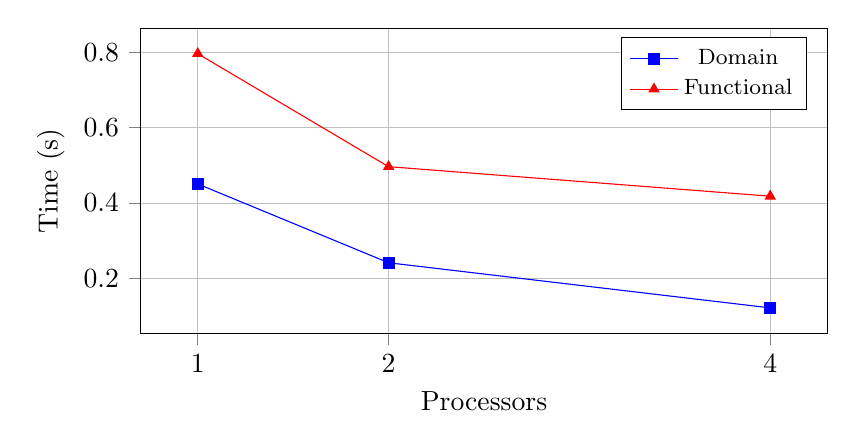
\begin{tikzpicture}
    \begin{axis}[
        standard,
        xlabel={Processors},
        ylabel={Time (s)},
        xtick={1,2,4},
        legend entries={Domain, Functional}
      ]
      \addplot[color=blue, mark=square*] coordinates {(1,0.450605) (2,0.241571) (4,0.121870)};
      \addplot[color=red, mark=triangle*] coordinates {(1,0.796236) (2,0.496460) (4,0.418110)};
    \end{axis}
  \end{tikzpicture}
  \caption{Execution time comparison on the Pine cluster.}
\end{figure}

\section{Performance Analysis}
\subsection{Scalability}
The domain decomposition model exhibits near-linear speedup as processors increase, whereas the functional model shows diminishing returns. The reorganization of loops ensured that cache misses were minimized, significantly improving performance compared to baseline implementations.

\subsection{Communication and Memory Constraints}
Functional decomposition faces severe memory constraints because each process must maintain a full copy of the sieve array, affecting scalability when running multiple tasks per node. Furthermore, the \texttt{MPI\_Reduce} step introduces substantial communication overhead compared to the optimized domain model, which requires only a minimal reduction for the final count.

\section{Conclusion}
The domain decomposition model, when optimized for cache efficiency and minimal communication, provides the most scalable solution for the Sieve of Eratosthenes. Functional decomposition, while useful for task distribution, is limited by its redundant memory usage and high reduction costs.

\newpage
\appendix
\section{Source Code: Domain Decomposition}
\lstinputlisting[language=C]{../domainSieve.c}

\newpage
\section{Source Code: Functional Decomposition}
\lstinputlisting[language=C]{../funcSieve.c}

\newpage
\section{Raw Results: Pine Cluster}
\lstinputlisting{../pine_sieve_results_121.txt}

\newpage
\section{Raw Results: Personal Cluster}
\lstinputlisting{../sieve_results.out}

\end{document}
